% !TeX root = ../main.tex

\chapter{字体、符号和排版}

\section{文本字体}

标题字体、\verb|\textbf{}|和\verb|\textsf{}|在Windows和Linux环境下表现不同。本文档默认在WSL环境编译。区别如表~\ref{tab-fonts-diff}~所示。

\begin{table}[htbp]
  \centering
  \caption{两种系统下的字体区别}
    \begin{tabular}{ccc}
    \toprule
          & Windows & Linux \\
    \midrule
    标题默认字体 & 黑体    & 宋体 \\
    \verb|\textsf{}| & 较大的等线字体 & 黑体 \\
    \verb|\textbf{}| & 黑体    & 宋体加粗 \\
    \bottomrule
    \end{tabular}%
  \label{tab-fonts-diff}%
\end{table}%

一般情况下强调字体使用\verb|\testbf{}|即可,在Linux环境下如果需要黑体需换成\verb|\textsf{}|。

\section{数学}

\subsection{公式环境}
数学公式环境可以使用:
\begin{itemize}
  \item \verb|align|:多行公式,默认居中,多列使用\&对齐。
  \item \verb|flalign|:多行公式,默认左对齐,多列使用\&对齐。
  \item \verb|gather|:多行公式,居中,无法多列及使用\&。
  \item \verb|equation|:单行公式。
\end{itemize}

下面是一个多栏公式的例子,使用\verb|flalign*|环境,注意第一列前用\&,其他列前使用\&\&,换行前再使用一次\&。
\begin{flalign*}
  &(1) \frac15\me^{5t}+C  
  &&(2) -\frac{(3-2x)^4}{8}+C 
  &&(3) -\frac12\ln|1-2x|+C  &\\
  &(4) -\frac12(2-3x)^{\frac23}+C 
  &&(5) -\frac{\cos ax}{a}-b\me^{\frac{x}{b}}+C 
  &&(6) -2\cos\sqrt{t}+C  \\
  &(7)-\frac12\me^{-x^2}+C 
  &&(8) \frac12 \sin(x^2)+C 
  &&(9) -\frac{\sqrt{2-3x^2}}{3}+C
\end{flalign*}
\begin{flalign*}
  &(1) \frac15\me^{5t}+C  
  &&(2) -\frac{(3-2x)^4}{8}+C &\\
  &(3) -\frac12\ln|1-2x|+C  
  &&(4) -\frac12(2-3x)^{\frac23}+C \\
  &(5) -\frac{\cos ax}{a}-b\me^{\frac{x}{b}}+C 
  &&(6) -2\cos\sqrt{t}+C  \\
  &(7)-\frac12\me^{-x^2}+C 
  &&(8) \frac12 \sin(x^2)+C \\
  &(9) -\frac{\sqrt{2-3x^2}}{3}+C
\end{flalign*}

在模板中有\verb|\allowdisplaybreaks[4]|允许较长的公式在中间换页。

\subsection{字体}

正文默认使用正体,数学环境默认使用斜体。

使用正体的情况:物理量的单位,单词缩写表示的下(上)标,一些常数($\mpi,\me,\mi$),微分算符$\md$,特殊函数($\sin,\ln$)。向量和矩阵使用粗斜体。

希腊字母的正体,使用\verb|\unicode-math|宏包(\verb|upgreek|宏包会改变字体),希腊字母加粗使用\verb|\symbf{}|,\verb|\symbfit{}|或\verb|symbfup{}|,效果如下:
\begin{gather*}
  \alpha \beta \gamma \delta \epsilon \varepsilon \zeta \eta \theta \vartheta \iota \kappa \lambda \mu \nu \xi o \pi \varpi \rho \varrho \sigma \varsigma \tau \upsilon \phi \varphi \chi \psi \omega
  A B \Gamma \varGamma \Delta \varDelta E Z H \Theta \varTheta I K \Lambda \varLambda M N \Xi \varXi O \Pi \varPi P \Sigma \varSigma T \Upsilon \varUpsilon \Phi \varPhi X \Psi \varPsi \Omega \varOmega 
\\
  (\text{up-})\upalpha \upbeta \upgamma \updelta \upepsilon  \upzeta \upeta \uptheta  \upiota \upkappa \uplambda \upmu \upnu \upxi \mathrm{o} \uppi  \uprho \upvarrho \upsigma  \uptau \upupsilon \upphi  \upchi \uppsi \upomega
  \upGamma     \upTheta   \upLambda  \upXi  \upPi   \upSigma  \upUpsilon  \upPhi   \upPsi  \upOmega  
\\
  (\mathrm{bfit})\symbfit{  \alpha \beta \gamma \delta \epsilon \varepsilon \zeta \eta \theta \vartheta \iota \kappa \lambda \mu \nu \xi o \pi \varpi \rho \varrho \sigma \varsigma \tau \upsilon \phi \varphi \chi \psi \omega
  A B \Gamma  \Delta  E Z H \Theta  I K \Lambda  M N \Xi  O \Pi  P \Sigma  T \Upsilon  \Phi  X \Psi  \Omega  }
\\
  (\mathrm{bf})\symbf{ \alpha \beta \gamma \delta \epsilon \varepsilon \zeta \eta \theta \vartheta \iota \kappa \lambda \mu \nu \xi o \pi \varpi \rho \varrho \sigma \varsigma \tau \upsilon \phi \varphi \chi \psi \omega
  A B \Gamma  \Delta  E Z H \Theta  I K \Lambda  M N \Xi  O \Pi  P \Sigma  T \Upsilon  \Phi  X \Psi  \Omega}
\\
  (\mathrm{bfup})\symbfup{ \alpha \beta \gamma \delta \epsilon \varepsilon \zeta \eta \theta \vartheta \iota \kappa \lambda \mu \nu \xi o \pi \varpi \rho \varrho \sigma \varsigma \tau \upsilon \phi \varphi \chi \psi \omega
  A B \Gamma  \Delta  E Z H \Theta  I K \Lambda  M N \Xi  O \Pi  P \Sigma  T \Upsilon  \Phi  X \Psi  \Omega}
\end{gather*}
小结:对小写希腊字母,\verb|up|前缀正体,\verb|\symbf{}|加粗斜体同\verb|\symbfit{}|,\verb|symbfup{}|加粗正体;对大写希腊字母,\verb|up|前缀正体同默认,\verb|var|前缀斜体,\verb|\symbf{}|加粗正体同\verb|\symbfup{}|,\verb|\symbfit{}|加粗斜体。

英文字母:
\begin{gather*}
  abcdefghijklmnopqrstuvwxyzABCDEFGHIJKLMNOPQRSTUVWXYZ
  \\
  (\mathrm{rm})\mathrm{abcdefghijklmnopqrstuvwxyzABCDEFGHIJKLMNOPQRSTUVWXYZ}
  \\
  (\mathrm{bf})\mathbf{abcdefghijklmnopqrstuvwxyzABCDEFGHIJKLMNOPQRSTUVWXYZ}
  \\
  (\mathrm{bf})\symbf{abcdefghijklmnopqrstuvwxyzABCDEFGHIJKLMNOPQRSTUVWXYZ}
  \\
  (\mathrm{bfit})\symbfit{abcdefghijklmnopqrstuvwxyzABCDEFGHIJKLMNOPQRSTUVWXYZ}
  \\
  (\mathrm{bb})\mathbb{abcdefghijklmnopqrstuvwxyzABCDEFGHIJKLMNOPQRSTUVWXYZ}
  \\
  (\mathrm{cal})\mathcal{abcdefghijklmnopqrstuvwxyzABCDEFGHIJKLMNOPQRSTUVWXYZ}
\end{gather*}

对于常用正体的字母,在配置文件中增加快捷键:
\begin{align*}
  \me^{\mi\mpi}+1=0 \qquad
  \mdd{y}{x}=\frac{\md }{\md x}f(x) \qquad
  \mdl x
\end{align*}

积分式的表示:
\begin{equation*}
  \int_a^b\! f(x)\,\md x = \left.F(x)\right|_a^b=F(x)\big|_a^b=F(x)\Big|_a^b=F(x)\bigg|_a^b
\end{equation*}

复数实部和虚部的表示:$z=a+b\mi,\Re(z)=a,\Im(z)=b$。
使用正体字母可以使用自定义命令\verb|\re|和\verb|\im|:$\re{z}=a,\im{z}=b$。


\subsection{其他符号}

文本中的分式$\myfrac{1}{2}$,虚位\phantom{字}命令;
$\ell \quad \nabla \quad 30^{\circ} $。

\subsection{定理环境}

\begin{theorem}[定理名字]
  这是一个定理。
\end{theorem}

\begin{definition}[定义名字]
  这是一个定义。
\end{definition}

\begin{proof}
  这是一个证明。
\end{proof}

\begin{example}
  这是一个例子。
\end{example}

\begin{solution}
  这是一个解。
\end{solution}



\section{排版}

\noindent  取消新段落前空格

加入一个水平线:

\noindent\rule{\textwidth}{0.5pt}

\subsubsection*{空格}

\begin{figure}[!htbp]
  \centering
  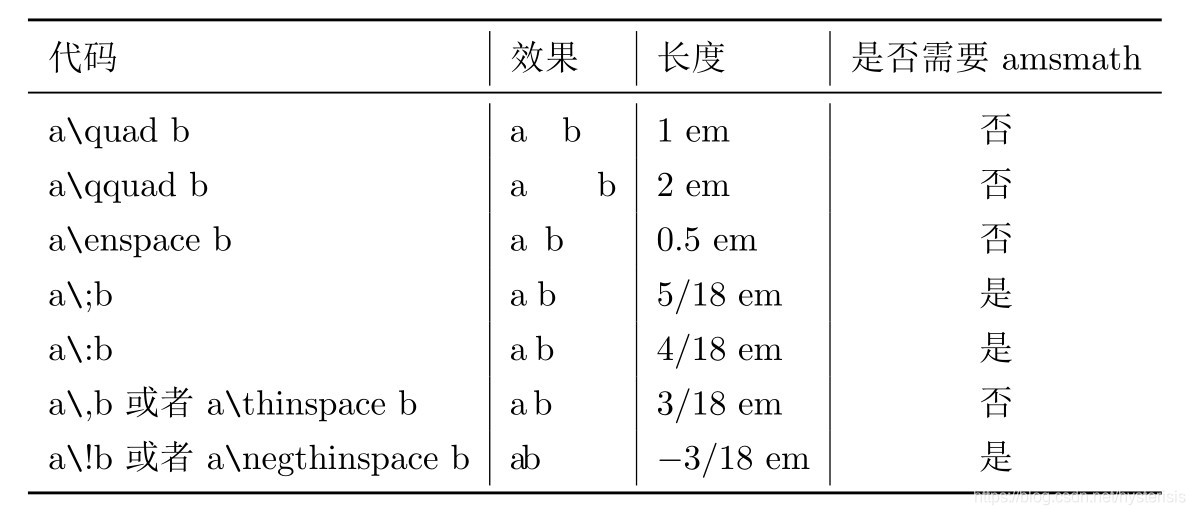
\includegraphics[width=85mm]{different-space.jpg}
  \caption{不同空格及其宽度}
  \label{fig-diff-space}
\end{figure}


使用\verb|a~b|:a~b不可分断空格,在此处不会换行。

使用\phantom{text}(同高宽)或\vphantom{text}(宽为0)或\hphantom{text}(高为0)产生指定占位字符长度的空白。
